In this section, we shall investigate two subsystems of
single agent \textsc{EviL}.

We first consider the following two fragments of the main grammar.
\begin{definition}
Define $\mathcal{L}^\boxminus (\Phi)$ as the fragment:
\[ \phi \ {::=} \  p \in \Phi \  | \  \phi
   \rightarrow \psi \  | \  \bot \  |
   \  \Box \phi \  | \  \boxminus \phi
 \  | \ 
   \circlearrowleft \]

Define $\mathcal{L}^\boxplus (\Phi)$ as the fragment:
\[ \phi \ {::=} \  p \in \Phi \  | \  \phi
   \rightarrow \psi \  | \  \bot \  |
   \  \Box \phi 
   \  | \  \boxplus \phi
 \  | \ 
   \circlearrowleft \]
\end{definition}

It is natural to wonder about \textsc{EviL} restricted to thee two
fragments.  After all, while ideas from Cartesian skepticism
naturally leads one to think about $\mathcal{L}^\boxminus(\Phi)$, as we saw in \S\ref{Descartes}, 
it is harder to motivate $\mathcal{L}^\boxplus (\Phi)$.
However, we regard each fragment as worthy of study in its own right.

Table \ref{table:axiomsII} gives the axioms systems for the two
fragments in question.  The system corresponding to the
$\mathcal{L}^\BM$ fragment is referred to as \textsc{EviL}$^\BM$, and
similarly the fragment corresponding to the $\mathcal{L}^\BP$ fragment
is referred to as \textsc{EviL}$^\BP$.

% For now, we shall observe that \textsc{EviL} extends \textsc{EviL}$^\BM$ and \textsc{EviL}$^\BP$.  In \S\ref{conservative-extension} we shall make this precise. 
\begin{table}
\begin{minipage}[b]{0.5\linewidth}
\centering
%\newcounter{rownum}
\setcounter{rownum}{0}
%\newcounter{rownum2}
\setcounter{rownum2}{0}
\begin{tabular}{|ll|}
\hline
  (\addtocounter{rownum}{1}\arabic{rownum})&$ \vdash \phi \rightarrow \psi \rightarrow \phi$\\
  (\addtocounter{rownum}{1}\arabic{rownum})&$ \vdash (\phi \rightarrow \psi \rightarrow \chi) \rightarrow (\phi
  \rightarrow \psi) \rightarrow \phi \rightarrow \chi$\\
  (\addtocounter{rownum}{1}\arabic{rownum})&$ \vdash (\neg \phi \rightarrow \neg \psi) \rightarrow \psi \rightarrow
  \phi$\\
  (\addtocounter{rownum}{1}\arabic{rownum})&$ \vdash \boxminus_X \phi \rightarrow \phi$\\
  (\addtocounter{rownum}{1}\arabic{rownum})&$ \vdash \boxminus_X \phi \rightarrow \boxminus_X \boxminus_X \phi$\\
  (\addtocounter{rownum}{1}\arabic{rownum})&$ \vdash p \rightarrow \boxminus_X p$\\
  (\addtocounter{rownum}{1}\arabic{rownum})&$ \vdash \neg p \rightarrow \boxminus_X \neg p$\\
  (\addtocounter{rownum}{1}\arabic{rownum})&$ \vdash \diamondsuit_X \phi \rightarrow \boxminus_X \diamondsuit_X \phi$\\
  (\addtocounter{rownum}{1}\arabic{rownum})&$ \vdash \Box_X \phi \rightarrow \Box_X \boxminus_Y \phi$\\
  (\addtocounter{rownum}{1}\arabic{rownum})&$ \vdash \phi \rightarrow \boxminus_X (\circlearrowleft_X \rightarrow
  \diamondsuit_X \phi)$\\
  (\addtocounter{rownum}{1}\arabic{rownum})&$ \vdash \circlearrowleft_X \rightarrow \boxminus_X \circlearrowleft_X$\\
  (\addtocounter{rownum}{1}\arabic{rownum})&$ \vdash \Box_X (\phi \rightarrow \psi) \rightarrow \Box_X \phi \rightarrow
  \Box_X \psi$\\
  (\addtocounter{rownum}{1}\arabic{rownum})&$ \vdash \boxminus_X (\phi \rightarrow \psi) \rightarrow \boxminus_X \phi
  \rightarrow \boxminus_X \psi$\\
(\addtocounter{rownum2}{1}\Roman{rownum2}) & 
 $\AxiomC{$\vdash \phi \to \psi$}
\AxiomC{$\vdash \phi$}
\BinaryInfC{$\vdash \psi$}
\DisplayProof$ \\ %& Modus Ponens\\[10pt]
(\addtocounter{rownum2}{1}\Roman{rownum2}) & 
 $\AxiomC{$\vdash \phi$}
\UnaryInfC{$\vdash \Box_X \phi$}
\DisplayProof$ \\ %& \multirow{3}{8.5cm}{Variations on necessitation}\\
(\addtocounter{rownum2}{1}\Roman{rownum2}) & 
 $\AxiomC{$\vdash \phi$}
\UnaryInfC{$\vdash \BB_X \phi$}
\DisplayProof$   \\
% (\addtocounter{rownum2}{1}\Roman{rownum2}) &
%  $\AxiomC{$\vdash \phi$}
% \UnaryInfC{$\vdash \BBI_X \phi$}
% \DisplayProof$  \\% [10pt]
\hline
\end{tabular}
\end{minipage}
\hspace{0.5cm}
\begin{minipage}[b]{0.5\linewidth}
 \centering
%\newcounter{rownum}
\setcounter{rownum}{0}
%\newcounter{rownum2}
\setcounter{rownum2}{0}
\begin{tabular}{|ll|}
\hline
  (\addtocounter{rownum}{1}\arabic{rownum})&$ \vdash \phi \rightarrow \psi \rightarrow \phi$\\
  (\addtocounter{rownum}{1}\arabic{rownum})&$ \vdash (\phi \rightarrow \psi \rightarrow \chi) \rightarrow (\phi
  \rightarrow \psi) \rightarrow \phi \rightarrow \chi$\\
  (\addtocounter{rownum}{1}\arabic{rownum})&$ \vdash (\neg \phi \rightarrow \neg \psi) \rightarrow \psi \rightarrow
  \phi$\\
  (\addtocounter{rownum}{1}\arabic{rownum})&$ \vdash \boxplus_X \phi \rightarrow \phi$\\
  (\addtocounter{rownum}{1}\arabic{rownum})&$ \vdash \boxplus_X \phi \rightarrow \boxplus_X \boxplus_X \phi$\\
  (\addtocounter{rownum}{1}\arabic{rownum})&$ \vdash p \rightarrow \boxplus_X p$\\
  (\addtocounter{rownum}{1}\arabic{rownum})&$ \vdash \neg p \rightarrow \boxplus_X \neg p$\\
  (\addtocounter{rownum}{1}\arabic{rownum})&$ \vdash \Box_X \phi \rightarrow \boxplus_X \Box_X \phi$\\
  (\addtocounter{rownum}{1}\arabic{rownum})&$ \vdash \Box_X \phi \rightarrow \Box_X \boxplus_Y \phi$\\
  (\addtocounter{rownum}{1}\arabic{rownum})&$ \vdash \phi \rightarrow \boxplus_X (\circlearrowleft_X \rightarrow
  \diamondsuit_X \phi)$\\
  (\addtocounter{rownum}{1}\arabic{rownum})&$ \vdash \neg \circlearrowleft_X \rightarrow \boxplus_X \neg
  \circlearrowleft_X$\\
  (\addtocounter{rownum}{1}\arabic{rownum})&$ \vdash \Box_X (\phi \rightarrow \psi) \rightarrow \Box_X \phi \rightarrow
  \Box_X \psi$\\
  (\addtocounter{rownum}{1}\arabic{rownum})&$ \vdash \boxplus_X (\phi \rightarrow \psi) \rightarrow \boxplus_X \phi
  \rightarrow \boxplus_X \psi$\\
(\addtocounter{rownum2}{1}\Roman{rownum2}) & 
 $\AxiomC{$\vdash \phi \to \psi$}
\AxiomC{$\vdash \phi$}
\BinaryInfC{$\vdash \psi$}
\DisplayProof$ \\ %& Modus Ponens\\[10pt]
(\addtocounter{rownum2}{1}\Roman{rownum2}) & 
 $\AxiomC{$\vdash \phi$}
\UnaryInfC{$\vdash \Box_X \phi$}
\DisplayProof$ \\ %& \multirow{3}{8.5cm}{Variations on necessitation}\\
% (\addtocounter{rownum2}{1}\Roman{rownum2}) & 
%  $\AxiomC{$\vdash \phi$}
% \UnaryInfC{$\vdash \BB_X \phi$}
% \DisplayProof$   \\
(\addtocounter{rownum2}{1}\Roman{rownum2}) &
 $\AxiomC{$\vdash \phi$}
\UnaryInfC{$\vdash \BBI_X \phi$}
\DisplayProof$  \\% [10pt]
\hline
\end{tabular}
\end{minipage}
\caption{Axiom system \textsc{EviL}$^\BM$ and \textsc{EviL}$^\BP$ respectively}
\label{table:axiomsII}
\end{table}

From these axioms, we shall define two sorts of \emph{\textsc{EviL}} models the correspond to the properties defined by
the above axiom systems.

% One should note that \textsc{EviL}$^\BM$ only induces properties on
% $\sqsupseteq$, and similarly \textsc{EviL}$^\BP$ only induces
% properties on $\sqsubseteq$. In each case, if either
% $\sqsubseteq$ or $\sqsupseteq$ has no defining axioms given by
% the logic then we shall simply assume that it is the inverse of its
% dual. 

% when we are restricting ourselves
% to thinking about $\mathcal{L}^\BM$, we 
\pagebreak

\begin{definition}The following properties specify 
\textbf{$\BM$\textsc{EviL}} and \textbf{$\BP$\textsc{EviL}} Kripke structures:

\begin{minipage}[b]{0.5\linewidth}
\begin{center}
\textbf{$\BM$\textsc{EviL}}
\end{center}
  \begin{enumerate}[label=\textup{(\emph{\Roman*})$^\BM$}, topsep=0.0in, parsep=0.075in]
    \item \label{MpI} $\sqsupseteq$ is reflexive
    \item \label{Mptrans} $\sqsupseteq$ is transitive 
    \item \label{Mpantisym} $\sqsupseteq$ is anti-symmetric
    \item \label{Mpreverse} $w \sqsupseteq v$ if and only if $v
    \sqsubseteq w$
   \item \label{Mislandiff} If $w \sqsupseteq v$ then ($w \in V (p)$ if and only if $v \in V (p)$)
     \item \label{MpV} $(R^{} \circ \sqsubseteq^{}) \subseteq
    R^{} $
     \item \label{MpVI} $(\sqsupseteq^{} \circ R^{}) \subseteq
R^{}$
     \item\label{MpVII} 
If $w \sqsupseteq v$ and $v \in P$ then $v R w$

    \item\label{MpIX} If $w \in P$ and $w \sqsupseteq v$ then $v
     \in P$
  \end{enumerate}
\end{minipage}
\hspace{0.5cm}
\begin{minipage}[b]{0.5\linewidth}
\begin{center}
\textbf{$\BP$\textsc{EviL}}
\end{center}
  \begin{enumerate}[label=\textup{(\emph{\Roman*})$^\BP$}, topsep=0.0in, parsep=0.075in]
    \item \label{PpI} $\sqsubseteq$ is reflexive
    \item \label{Pptrans} $\sqsubseteq$ is transitive 
    \item \label{Ppantisym} $\sqsubseteq$ is anti-symmetric
    \item \label{Ppreverse} $w \sqsubseteq v$ if and only if $v \sqsupseteq w$
   \item \label{Pislandiff} If $w \sqsubseteq v$ then ($w \in V (p)$ if and only if $v \in V (p)$)
     \item \label{PpV}  $(R^{} \circ \sqsubseteq^{}) \subseteq
    R^{} $
     \item \label{PpVI} $(\sqsubseteq^{} \circ R^{}) \subseteq
 R^{}$
     \item\label{PpVII} If $w \sqsubseteq v$ and $v \in P$ then $v
       R w$

    \item\label{PpIX} If $w \nin P$ and $w \sqsubseteq v$ then $v
     \nin P$
  \end{enumerate}
\end{minipage}
\end{definition}

Exactly as in the case of the \textsc{EviL} Kripke structures we
introduced in \S\ref{kripke}, we may naturally visualize certain
properties in commutative diagrams:
\begin{bul}
%\item Properties \ref{MpV} and \ref{PpV} are depicted in
%Fig. \ref{fig:dupcommut1}
\item  Properties \ref{MpV} and \ref{PpV} are depicted as
Fig. \ref{fig:dupcommut1}, which is the same as Fig. \ref{fig:commut1}
\item  Property \ref{MpVI} is depicted as
Fig. \ref{fig:dupcommut2}, which is the same as Fig. \ref{fig:commut2}
\item  Property \ref{PpVI} is depicted as
Fig. \ref{fig:dupcommut3}, which is the same as Fig. \ref{fig:commut3}
\end{bul}

\begin{figure}[ht]
\centering
% \subfigure[--\ \ref{MpV} \& \ref{PpV}\ -- ]{
%   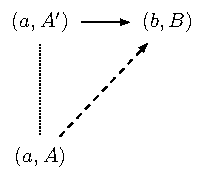
\includegraphics[]{commutative/commutative1.pdf}
% %\caption{A fairly simple example}
% \label{fig:dupcommut1}
% }
% \hspace{1cm}
\subfigure[--\ \ref{MpVI} \& \ref{PpVI} \ -- ]{
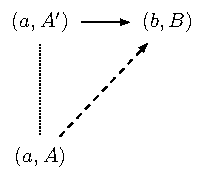
\includegraphics[]{commutative/commutative1.pdf}
\label{fig:dupcommut1}
}
\subfigure[--\ \ref{MpVI}\ -- ]{
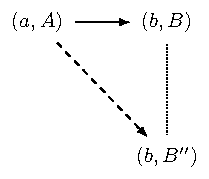
\includegraphics[]{commutative/commutative3.pdf}
\label{fig:dupcommut2}
}
\hspace{1cm}
\subfigure[--\ \ref{PpVI}\ --]{
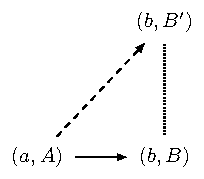
\includegraphics[]{commutative/commutative2.pdf}
\label{fig:dupcommut3}
}
\caption{Visualizations of the relationships in Proposition \ref{evil_models}}
\end{figure}

We may recall that the commutative diagrams depicted split
the original \textsc{EviL} property \ref{pV};  this is not coincidental.
By elementary reasoning we may observe that every 
partly \textsc{EviL} Kripke structure 
(and hence, every \textsc{EviL} Kripke structure) is  
both $\BM$\textsc{EviL} and $\BP$\textsc{EviL}.  In fact, the logical differences between partly
\textsc{EviL}, $\BM$\textsc{EviL}, and $\BP$\textsc{EviL} properties respectively may be summarized as follows:
\begin{bul}
\item $\BM$\textsc{EviL} and $\BP$\textsc{EviL} Kripke structures \emph{strengthen} \ref{ppVII} to
\ref{MpVII} and \ref{PpVII}.  Note that in the presence of the other properties
of $\BM$\textsc{EviL} and $\BP$\textsc{EviL} Kripke structures,
we may observe that \ref{MpVII} and \ref{PpVII} are logically equivalent.
\item $\BM$\textsc{EviL} and $\BP$\textsc{EviL} Kripke structures \emph{weaken} \ref{ppVI} to
\ref{MpVI} and \ref{PpVI}, respectively.
\item With the exception of \ref{MpVI} and
\ref{PpVI}, the $\BM$\textsc{EviL} properties are logically
equivalent to the $\BP$\textsc{EviL} properties.
\end{bul}

Hence, just as the proof of abstract completeness of \textsc{EviL}
involved producing \textsc{EviL} bisimilar completions of partly
\textsc{Evil} 
Kripke structures using the operator $\invis$, 
the proof of the abstract completeness of
\textsc{EviL}$^\BM$ and \textsc{EviL}$^\BP$ shall involve producing
partly \textsc{EviL} bisimilar completions
% , using two new operators
% $\ominus$ and $\oplus$, which we shall introduce shortly.  

Before turning to bisimulation, we shall first prove abstract
completeness for \textsc{EviL}$^\BM$ and \textsc{EviL}$^\BP$ and their
respective classes of Kripke structures.

\begin{definition}\label{BM-BPEviL-Vdash}
We shall write
\[ \Gamma \Vdash_{\BM\textup{\textsc{EviL}}} \phi \]
to mean that for all $\BM$\textsc{EviL}  Kripke structures
$\mathbb{M} = \langle W, R, \sqsubseteq, \sqsupseteq, V, P \rangle$,
for all worlds $w \in W$ if $\mathbb{M},w \Vdash \Gamma$ then
$\mathbb{M} \Vdash \phi$.

Moreover, we shall write
\[ \Gamma \Vdash_{\BP\textup{\textsc{EviL}}} \phi \]
to mean the same for all $\BP$\textsc{EviL}  Kripke structures.
\end{definition}

\begin{theorem}[${\BM/\BP}$\textsc{EviL} 
Strong Soundness and Completeness]\label{BMBPbadcompleteness}
\begin{eqnarray*}
& \Gamma \vdash_{\textsc{EviL}^\BM} \phi\textup{ if and only if }\Gamma
\Vdash_{\BM\textup{\textsc{EviL}}} \phi \\
& \& \\
& \Gamma \vdash_{\textsc{EviL}^\BP} \phi\textup{ if and only if }\Gamma
\Vdash_{\BP\textup{\textsc{EviL}}} \phi 
\end{eqnarray*}
\end{theorem}
\begin{proof}
  The proof of these two propositions, in each case, proceeds exactly as in the proof of Theorem
  \ref{partly-evil-completeness} from \S\ref{abstraction}. In each
  case we perform the usual canonical model construction that is used
  in modal logic.  
  Rather than rehash that proof, here
  we simply list how we may infer the desired properties we attribute
  to these canonical models.  At the risk of being slightly redundant, we have chosen to
  present the arguments for both logics, even though they are highly symmetric:

\begin{minipage}[b]{0.5\linewidth}
\begin{center}
\textbf{$\BM$\textsc{EviL}}
\end{center}
  \begin{empt}
    \item \ref{MpI} corresponds to the \textsc{EviL}$^\BM$ axiom \eqref{Mrefl}
    \item \ref{Mptrans} corresponds to the \textsc{EviL}$^\BM$ axiom \eqref{Mtrans}
    \item \ref{Mpreverse} -- Since the canonical model construction in
      this case does not specify $\sqsubseteq$, we shall define 
     $w \sqsubseteq  v$ if and only if $v \sqsupseteq w$
   \item \ref{Mislandiff} corresponds to the \textsc{EviL}$^\BM$
     axioms \eqref{Misland1} and \eqref{Misland2}
    \item \ref{MpV} corresponds to the \textsc{EviL}$^\BM$
     axiom \eqref{Mdownconceive}
    \item \ref{MpIX} corresponds to the \textsc{EviL}$^\BM$
     axiom \eqref{MaxpIX}
    \item \ref{Mpantisym} -- 
     Just as in the case of the proof of Theorem 
    \ref{partly-evil-completeness}, this step follows from the above
  properties, the Truth Lemma, and an inductive argument
     \item \ref{MpVI} corresponds to the \textsc{EviL}$^\BM$
     axiom \eqref{MaxpVI}
     \item \ref{MpVII} corresponds to the \textsc{EviL}$^\BM$
     axiom \eqref{MaxpVII}
  \end{empt}
\end{minipage}
\hspace{0.5cm}
\begin{minipage}[b]{0.5\linewidth}
\begin{center}
\textbf{$\BP$\textsc{EviL}}
\end{center}
  \begin{empt}
    \item \ref{PpI} corresponds to the \textsc{EviL}$^\BP$ axiom \eqref{Mrefl}
    \item \ref{Pptrans} corresponds to the \textsc{EviL}$^\BP$ axiom \eqref{Mtrans}
    \item \ref{Ppreverse} -- Since the canonical model construction in
      this case does not specify $\sqsupseteq$, we shall define 
     $w \sqsupseteq  v$ if and only if $v \sqsubseteq w$
   \item \ref{Pislandiff} corresponds to the \textsc{EviL}$^\BP$
     axioms \eqref{Misland1} and \eqref{Misland2}
    \item \ref{PpV} corresponds to the \textsc{EviL}$^\BP$
     axiom \eqref{Mdownconceive}
    \item \ref{PpIX} corresponds to the \textsc{EviL}$^\BP$
     axiom \eqref{MaxpIX}
    \item \ref{Ppantisym} -- 
     Just as in the case of the proof of Theorem 
    \ref{partly-evil-completeness}, this step follows from the above
  properties, the Truth Lemma, and an inductive argument
     \item \ref{PpVI} corresponds to the \textsc{EviL}$^\BP$
     axiom \eqref{MaxpVI}
     \item \ref{PpVII} corresponds to the \textsc{EviL}$^\BP$
     axiom \eqref{MaxpVII}
  \end{empt}
\end{minipage}
\end{proof}

With the previous completeness theorem, we shall give two constructions which
provide bisimular partly \textsc{EviL} completions of 
both $\BM$\textsc{EviL} and $\BP$\textsc{EviL} Kripke
structures.

\begin{mydef}[$\ominus$ and $\oplus$ Bisimulators]
\label{Plus-Minus-Bisimulators}
Let $\mathbb{M}$ be a Kripke model, then define:

\begin{minipage}[b]{0.5\linewidth}
$$\ominus^\mathbb{M} := \langle W^{\ominus}, R^{\ominus}, \sqsubseteq^{\ominus},
\sqsupseteq^{\ominus}, V^{\ominus}, P^{\ominus} \rangle$$ 
where:
 \begin{eqnarray*}
 W^\ominus & := &  \sqsupseteq^{\mathbb{M}} \\
 V^\ominus(p) & := &  \{(w,v) \in   W^\ominus \ |\ v \in V^{\mathbb{M}} \}\\
 P^\ominus & := & \{(w,v) \in   W^\ominus \ |\ v \in V^{\mathbb{M}} \} \\
 R^\ominus & := &  \{((w,v), (t,u)) \in   (W^\ominus)^2 \ |\ v
 R^\mathbb{M} t\ \&\ \\
& & \hspace{4.36cm} v
 R^\mathbb{M} u \}  \\
 \sqsupseteq^\ominus & := &  \{((w,v), (w,u)) \in   (W^\ominus)^2 \ |\ v \sqsupseteq^{\mathbb{M}} u \}  \\
 \sqsubseteq^\ominus & := &  \{((w,v), (w,u)) \in   (W^\ominus)^2 \ |\ v \sqsubseteq^{\mathbb{M}} u \}  
 \end{eqnarray*}
\end{minipage}
\hspace{0.5cm}
\begin{minipage}[b]{0.5\linewidth}
$$\oplus^\mathbb{M} := \langle W^{\oplus}, R^{\oplus}, \sqsubseteq^{\oplus},
\sqsupseteq^{\oplus}, V^{\oplus}, P^{\oplus} \rangle$$ 
where:
 \begin{eqnarray*}
 W^\oplus & := &  \sqsubseteq^{\mathbb{M}} \\
 V^\oplus(p) & := &  \{(w,v) \in   W^\oplus \ |\ v \in V^{\mathbb{M}} \}\\
 P^\oplus & := & \{(w,v) \in   W^\oplus \ |\ v \in V^{\mathbb{M}} \} \\
 R^\oplus & := &  \{((w,v), (t,u)) \in   (W^\oplus)^2 \ |\ v
 R^\mathbb{M} t\ \&\ v R^\mathbb{M} u \}  \\
 \sqsupseteq^\oplus & := &  \{((w,v), (w,u)) \in   (W^\oplus)^2 \ |\ v \sqsupseteq^{\mathbb{M}} u \}  \\
 \sqsubseteq^\oplus & := &  \{((w,v), (w,u)) \in   (W^\oplus)^2 \ |\ v \sqsubseteq^{\mathbb{M}} u \}  
 \end{eqnarray*}
\end{minipage}
\end{mydef}

Our intuition for the above construction comes from the following proposition:
\begin{mydef}
Let $\downarrow w := \{ v \in W \ |\ w \sqsupseteq v\}$, which is the
\textbf{downset} of $w$.

Let $\uparrow w := \{ v \in W \ |\ w \sqsupseteq v\}$, which is the
\textbf{upset} of $w$.
\end{mydef}

\begin{lemma}[Downset/Upset Lemma]\label{downset-upset-lemma}\ \\
\begin{minipage}[b]{0.5\linewidth}
Let $\mathbb{M}$ be a partly $\textsc{EviL}^\BM$ Kripke structure. We have:
\begin{enumerate}[label=\textup{(\emph{\arabic*})$^\BM$},
  topsep=0.075in, parsep=0.075in]
  \item For all $w$, $w \in \downarrow w$
  \item $w R v$ if and only if $w R \downarrow v$
  \item if $w \in \downarrow v$ then $w \in V(p)$ if and only if $v
    \in V(p)$
  \item $v \sqsupseteq w$ and $w \in P$ implies $w R \downarrow v$
\end{enumerate}
\end{minipage}
\hspace{0.5cm}
\begin{minipage}[b]{0.5\linewidth}
Let $\mathbb{M}$ be a partly $\textsc{EviL}^\BP$ Kripke structure.  We have:
\begin{enumerate}[label=\textup{(\emph{\arabic*})$^\BP$}, topsep=0.075in, parsep=0.075in]
  \item For all $w$, $w \in \uparrow w$
  \item $w R v$ if and only if $w R \uparrow v$
  \item if $w \in \uparrow v$ then $w \in V(p)$ if and only if $v
    \in V(p)$
  \item $v \sqsupseteq w$ and $w \in P$ implies $w R \uparrow v$
\end{enumerate}
\end{minipage}
\end{lemma}
\begin{proof}\ \\
\begin{minipage}[b]{0.5\linewidth}
\begin{enumerate}[label=\textup{(\emph{\arabic*})$^\BM$},
  topsep=0.075in, parsep=0.075in]
  \item Follows from property \ref{MpI}
  \item Follows from properties \ref{MpI} and \ref{MpVI}
  \item Follows from property \ref{Mislandiff}
  \item Follows from properties \ref{MpVI} and \ref{MpVII}
\end{enumerate}
\end{minipage}
\hspace{0.5cm}
\begin{minipage}[b]{0.5\linewidth}
\begin{enumerate}[label=\textup{(\emph{\arabic*})$^\BP$},
  topsep=0.075in, parsep=0.075in]
 \item Follows from property \ref{PpI}
  \item Follows from properties \ref{PpI} and \ref{PpVI}
  \item Follows from property \ref{Pislandiff}
  \item Follows from properties \ref{PpVI} and \ref{PpVII}
\end{enumerate}
\end{minipage}
\end{proof}

We now can state the central idea behind $\ominus$ and $\oplus$.
Essentially, in $\ominus$ and $\oplus$  we shall force the
islands of each of the structures we construct to correspond to the downsets and
upsets of the original $\BM$\textsc{EviL} and $\BP$\textsc{EviL}
structures, respectively.  We note that in many respects, Lemma
\ref{downset-upset-lemma} illustrates that downsets and upsets are
similar in many respects to islands, just as we saw in Lemma
\ref{island}, the Island Lemma, from \S\ref{islands}. In $\ominus$, each world has as its first coordinate which downset it
belongs to, and similarly for $\oplus$.  As a consequence,
$\sqsupseteq$ and $\sqsubseteq$ end up being the set of worlds in each
of these constructions.

To see that $\ominus$ and $\oplus$ are the completions we want, we shall see that $\oplus$ and $\ominus$ give rise to special
bisimulations, which each preserve the formulae of
$\mathcal{L}^\BM(\Phi)$ and $\mathcal{L}^\BP(\Phi)$.  We will next
see that if $\mathbb{M}$ is $\BM$\textsc{EviL} then $\ominus$ is
partly \textsc{EviL}, and likewise if $\mathbb{M}$ is
$\BP$\textsc{EviL} then $\ominus$  is partly \textsc{EviL}.  Since in
the case of the logics \textsc{EviL}$^\BM$ and \textsc{EviL}$^\BP$ we
are only concerned with fragments of the main language, the limited
bisimulations we will deploy will be sufficient for our purposes.

\begin{mydef}
A relation $Z$ is called a $\BM$-bisimulation between $\mathbb{M}$ and
$\mathbb{M}'$, with type annotation $Z:\mathbb{M}\leftrightarroweq^\BM\mathbb{M}'$, if it satisfies the letter
conditions, as well as the back and forth conditions for $R$ and
$\sqsupseteq$, but not necessarily $\sqsubseteq$.

A $Z$ relation is called a $\BP$-bisimulation is the same, with type
annotation $Z:\mathbb{M}\leftrightarroweq^\BP\mathbb{M}'$, only in
this case weenforce the back and forth conditions for $R$ and
$\sqsubseteq$, but not necessarily $\sqsupseteq$.
\end{mydef}

The following is a trivial consequence of \emph{The Fundamental
  Theorem of Bisimulations}, Theorem \ref{fundamental-bisim-theorem},
that we gave in \ref{completely-evil}:

\begin{proposition}\label{bmbpbisimprop}
If $Z:\mathbb{M}\leftrightarroweq^\BM\mathbb{M}'$, then if $\phi \in
\mathcal{L}^\BM(\Phi)$ and $w Z v$ then $\mathbb{M},w \Vdash \phi \iff
\mathbb{M}',v \Vdash \phi$.

If $Z:\mathbb{M}\leftrightarroweq^\BP\mathbb{M}'$, then if $\phi \in
\mathcal{L}^\BP(\Phi)$ and $w Z v$ then $\mathbb{M},w \Vdash \phi \iff \mathbb{M}',v \Vdash \phi$.
\end{proposition}

As asserted, $\ominus$ and $\oplus$ each give rise to
$\BM$-bisimilar and $\BP$-bisimilar Kripke structures, respectively:

\begin{lemma}\label{bmbpbisimlemma}
Let $\mathbb{M}$ be a Kripke structure.

If $\sqsupseteq$ is reflexive and transitive, then $Z: \mathbb{M}
\leftrightarroweq^\BM \ominus^\mathbb{M}$ where $w Z (u,w)$ for all $u \in \mathbb{M}$

In the same vain, if $\sqsupseteq$ is reflexive and transitive, then
again $Z: \mathbb{M}
\leftrightarroweq^\BP \ominus^\mathbb{M}$ where $w Z (u,w)$ for all $u \in \mathbb{M}$
\end{lemma}
\begin{proof}
The two proofs are entirely analogous, so we shall only prove for
$\ominus$.
\begin{bul}
  \item Proposition letters and $P$:  Simply note that we defined
\[ (u,w) \in V^\ominus(p) \iff w \in V^{\mathbb{M}}(p) \]
And similarly for $P$
\item $R$ forth:  Assume that $w R^\mathbb{M} v$ and $w Z (u,w)$.
  Since we are assume that $\sqsubseteq$ is reflexive then we know
  that $(v,v) \in W^\ominus$, hence $v Z (v,v)$ and $(u,w)
  R^\mathbb{M} (v,v)$ as per definition.
\item $R$ back:  Assume that $(u,w) R^\ominus (t,v)$ and $w Z (u,w)$;
  by construction it must be that $w R^{\mathbb{M}} v$.
\item $\sqsupseteq$ forth:  Assume that $w \sqsupseteq^{\mathbb{M}} v$ and $w Z
  (u,w)$.  It must then be that $u \sqsupseteq^{\mathbb{M}} w$ by construction,
  whence by transitivity we know that $u \sqsupseteq^{\mathbb{M}} v$ and thus
  $(u,v) \in W^\ominus$.  So $v Z (u,v)$ and moreover $(u,w)
  \sqsupseteq^\ominus (u,v)$ by construction, which suffices.
\item $\sqsupseteq$ back: As with the case for $R$ back, this follows
  by construction.
\end{bul}
\end{proof}

We now show that $\ominus$ and $\oplus$ really are adequate completions:

\begin{lemma}[$\BM/\BP$ Completion]\label{bm-bp completion}\ \\
If $\mathbb{M}$ is $\BM$\textsc{Evil}, then $\ominus$ is
partly \textsc{EviL}

Likewise, if $\mathbb{M}$ is $\BP$\textsc{EviL}, then $\oplus$ is
partly \textsc{EviL}
\end{lemma}
\begin{proof}
Since the proof involves many steps, we shall economize on space by
only proving for $\ominus$, since $\oplus$ is similar.
\begin{enumerate}[label=\textup{(\emph{\Roman*})$'$}, topsep=0.0in,
  parsep=0.075in]
\item asserts $\sqsubseteq^\ominus$ is reflexive.  This follows by
  construction since $\sqsubseteq^\mathbb{M}$ is reflexive, as per
  \ref{MpI} and \ref{Mpreverse}.
\item asserts $\sqsubseteq^\ominus$ is transitive.  This follows by
  construction since $\sqsubseteq^\mathbb{M}$ is transitive, as per
  \ref{Mptrans} and \ref{Mpreverse}.
% \item follows from the fact that $\mathbb{M}$ makes true \ref{Mptrans}, hence
%   $\sqsubseteq^\ominus$ is transitive by construction, as desired.
\item asserts that $\sqsubseteq^\ominus$ is a partial order. To show
  this, by the above all we have to show is that $\sqsubseteq^\ominus$ is anti-symmetric.  
  We shall use that $\mathbb{M}$ makes true \ref{Mpantisym} and \ref{Mpreverse}. 
  
  Assume that $(a,b) \sqsubseteq^{\ominus} (c,d)$ and $(b,a)
  \sqsubseteq^{\ominus} (d,c)$.  We want to show that $a =d$ and $b
  =c$.    By construction it must be that $a = d$.  
  We also have by construction that $b \sqsubseteq^{\mathbb{M}} c$, $c
  \sqsubseteq^{\mathbb{M}} b$.  
  As we noted, $\sqsubseteq^{\mathbb{M} }$ is anti-symmetric by \ref{Mpantisym} and \ref{Mpreverse}, 
  hence $b = c$. 
\item asserts that $\sqsupseteq^\ominus$ is the reverse of
  $\sqsubseteq^\ominus$, which follows directly by construction
\item asserts that ``if $w \sqsubseteq^\ominus v$ then ($w \in V (p)$
  if and only if $v \in V (p)$).''  This follows by construction and
  \ref{Mislandiff} for $\mathbb{M}$.
\item asserts  \[(R^{\ominus} \circ \sqsubseteq^{\ominus}) \subseteq
    R^{\ominus}.\]
As above, $\ominus$ inherits this property from $\mathbb{M}$, which
obeys \ref{MpV}.

\item asserts 
\begin{eqnarray*}
& (\sqsubseteq^\ominus \circ R) \subseteq R^\ominus \\
& \& \\
&    (\sqsupseteq^\ominus \circ R^\ominus) \subseteq R^\ominus.
\end{eqnarray*}
Since $\mathbb{M}$ obeys \ref{MpVI}, we have that 
\[ ( \sqsupseteq^{\ominus} \circ R^{\ominus}) \subseteq R^{\ominus} \]

So it suffices to show that if $(s,w) R^\ominus (t,u) \sqsupseteq^\ominus (t,v)$
then $w R^\ominus v$.  We can see by the definition of $\ominus$ that
all we have to show is that $w R^\mathbb{M} v$.  
With our assumptions, we can see by construction that we know the following two things:
\begin{eqnarray*}
 & w R^\mathbb{M} t   \\
& \& \\
& v \in \downarrow t
\end{eqnarray*}  
However, we know from Lemma
\ref{downset-upset-lemma}, the Downset/Upset Lemma, that if $w
R^\mathbb{M} t$ then $ w R^\mathbb{M} \downarrow t$, which means that
$w R^\mathbb{M} v$ as desired.
\item We must show ``If $(v,w) \in P^\ominus$ then $(v,w)
    R^\ominus (v,w)$.''  So assume that $(v,w) \in P^\ominus$.  By
    construction we must show that $w R^{\mathbb{M}} v$ and $w R^{\mathbb{M}} w$

Since $(v,w) \in W^\ominus$ then by construction we know $w
\sqsubseteq^\mathbb{M} v$.   Since $(v,w) \in P^\ominus$, then
evidently $w
    \in P^{\mathbb{M}}$.  So by \ref{MpVII} we know that $w
    R^{\mathbb{M}} v$.  

We may also note by \ref{MpI} that $w
    \sqsubseteq w$, so applying our assumptions and \ref{MpVII}
    again we have that $w R^\mathbb{M} w$, which suffices.
\item The last thing to show is ``If $w \in P_X^\ominus$ and $w \sqsupseteq_X^\ominus v$ then $v
    \in P_X^\ominus$.'' However, this follows immediately by
    construction from \ref{MpIX}.
\end{enumerate}
\end{proof}

With the above, we have what we need to prove the central result
regarding these subsystems:

\begin{theorem}[$\BM/\BP$ Embedding, Soundness and
  Completenesses]\label{lotsocompleteness}\ \\
\begin{minipage}[b]{0.5\linewidth}
Assume $\Gamma \cup \{\phi\} \subseteq \mathcal{L}^\boxminus(\Phi,\mathcal{A})$. The following are equivalent:
\begin{align*}
\Gamma \vdash_{\textsc{EviL}^\BM} \phi & \iff \Gamma
\Vdash_{\BM\textup{\textsc{EviL}}} \phi \\
 & \iff \Gamma \Vdash_{p\textup{\textsc{EviL}}} \phi \\
 & \iff \Gamma \Vdash_{\textup{\textsc{EviL}}} \phi \\
 & \iff \Gamma \vdash_{\textup{\textsc{EviL}}} \phi
\end{align*}
\end{minipage}
\hspace{0.5cm}
\begin{minipage}[b]{0.5\linewidth}
Assume $\Gamma \cup \{\phi\} \subseteq \mathcal{L}^\BP(\Phi,\mathcal{A})$. The following are equivalent:
\begin{align*}
\Gamma \vdash_{\textsc{EviL}^\BP} \phi & \iff \Gamma
\Vdash_{\BP\textup{\textsc{EviL}}} \phi \\
 & \iff \Gamma \Vdash_{p\textup{\textsc{EviL}}} \phi \\
 & \iff \Gamma \Vdash_{\textup{\textsc{EviL}}} \phi \\
 & \iff \Gamma \vdash_{\textup{\textsc{EviL}}} \phi
\end{align*}
\end{minipage}
\end{theorem}
\begin{proof}
As before, we only show the result for \textsc{EviL}$^\BM$.

The only nontrivial equality is $\Gamma \vdash_{\textsc{EviL}^\BM} \phi \iff \Gamma
\Vdash_{p\textup{\textsc{EviL}}} \phi$. It is straightforward to verify that $\Gamma \vdash_{\textsc{EviL}^\BM} \phi \Longrightarrow \Gamma
\Vdash_{p\textup{\textsc{EviL}}} \phi$, since this is just a
soundness result.  To show the converse, we shall establish the
contrapositive.  Assume that $\Gamma \nvdash_{\textsc{EviL}^\BM}
\phi$. By Theorem \ref{BMBPbadcompleteness}, there is some $\BM\textsc{EviL}$ Kripke structure
$\mathbb{M}$ with a world $w$ such that $\mathbb{M},w \Vdash \Gamma$
and $\mathbb{M},w \nVdash \phi$.  Since
$\mathbb{M}\leftrightarroweq^\BM\ominus^\mathbb{M}$, then by our
grammar restriction assumptions, Proposition \ref{bmbpbisimprop} and
Lemma \ref{bmbpbisimlemma} we have $\ominus^\mathbb{M},(w,w) \Vdash
\Gamma$ and $\ominus^\mathbb{M},(w,w) \nVdash
\phi$.  By \ref{bm-bp completion} we know that $\ominus$ is partly
\textsc{EviL}. which suffices our claim.

Hence we have:

\begin{align*}
\Gamma \vdash_{\textsc{EviL}^\BM} \phi & \iff \Gamma
\Vdash_{\BM\textup{\textsc{EviL}}} \phi & \text{by Theorem \ref{BMBPbadcompleteness}}\\
 & \iff \Gamma \Vdash_{p\textup{\textsc{EviL}}} \phi & \textup{by our
   reasoning above}\\
 & \iff \Gamma \vdash_{\textup{\textsc{EviL}}} \phi & \textup{by
   Theorem \ref{partly-evil-completeness} from \S\ref{abstraction}}\\
 & \iff \Gamma \Vdash_{\textup{\textsc{EviL}}} \phi & \textup{by
   Theorem \ref{evil-completeness} from \S\ref{Abstract-Completeness}}
\end{align*}
\end{proof}

With the above abstract completeness result, by the reasoning we
provided in \S\ref{taking-stockII}, we can employ our abstract semantics
to avoid dealing directly with the \textsc{EviL} concrete semantics,
and easily arrive at couple lemmas:  
% The above also
% affords us numerous lemmas regarding these fragments:

\begin{lemma}[$\BM/\BP$ Weak Soundness and Completeness] \ \\
If $\Gamma\subseteq_\omega \mathcal{L}^\boxminus(\Phi,\mathcal{A})$ is
finite, then 
\begin{align*}
\Gamma \vdash_{\textsc{EviL}^\BM} \phi & \iff \Gamma
\VDash \phi
\end{align*}

Likewise, if $\Gamma\subseteq_\omega \mathcal{L}^\BP(\Phi,\mathcal{A})$ is finite, then 
\begin{align*}
\Gamma \vdash_{\textsc{EviL}^\BP} \phi & \iff \Gamma
\VDash \phi
\end{align*}
\end{lemma}
\begin{proof}
This follows by Theorem \ref{lotsocompleteness} above and Lemma \ref{coincide} in \S{taking-stockII}.
\end{proof}

\begin{theorem}[$\BM/\BP$ Small Model Property]
If $\phi$ is ${\BM\textsc{EviL}}$ or ${\BP\textsc{EviL}}$ satisfiable,
 then it is finitely satisfiable in a \textsc{EviL} Kripke structure
 with $O(EXP2(|\phi|))$ worlds.
\end{theorem}
\begin{proof}
This follows by Theorem \ref{lotsocompleteness} above and our previous
small model property we established in Theorem
\ref{small-model-property} in \S\ref{small-model}.
\end{proof}

\begin{theorem}[$\BM/\BP$ Decidability]
The decision problems for $\vdash_{\textsc{EviL}^\BM} \phi$ and
$\vdash_{\textsc{EviL}^\BP} \phi$ have time complexity bounded
above by $O(EXP3(|\phi|))$.
\end{theorem}
\begin{proof}
As before, this is an application of Theorem \ref{lotsocompleteness} 
and Theorem \ref{evil-decidability}.
\end{proof}

As a final note, we should mention why these results do not generalize
to more than one agent.  The central issue is precisely that the
observation that downsets and upsets can play the role of islands, as
we asserted in Lemma \ref{downset-upset-lemma}, the Downset/Upset
Lemma, do not generalize to multiple agents.   

The central issue is that intuitions about how $\PP$ functions in the
single agent case do not extend to multiple agents. Specifically,
consider the plausible extension of $\textsc{EviL}^\BM$ and $\textsc{EviL}^\BP$
with the following two axioms from ordinary multi-agent \textsc{EviL}:
\begin{eqnarray*} 
& \vdash \Box_X \phi \to \Box_X\BM_Y\phi \\
& \& \\
& \vdash \Box_X \phi \to \Box_X\BP_Y\phi 
\end{eqnarray*}

We may then plausibly extend our notion of downset and upset
\begin{align*}
\downarrow^\ast w & := \left\{ v \in W\ \left| \ w \left(\bigcup_{X\in
    \mathcal{A}}\sqsupseteq_X\right)^\ast\right. v\right\}\\
\uparrow^\ast w & := \left \{ v \in W\ \left| \ w \left(\bigcup_{X\in
    \mathcal{A}}\sqsubseteq_X\right)^\ast\right. v\right\}
\end{align*}
With this, we would indeed get that ``if $wR_Xv$ then $w R_X
\downarrow^\ast v$'' for $\BM$\textsc{EviL} Kripke structures and the
dual for $\BP$\textsc{EviL} Kripke structures.  

We stumble when we try
to enforce ``if $w \in \downarrow^\ast v$ and $w \in P_X$ then $w
R_X \downarrow^\ast v$.''  Somehow, we would need to enforce that if
there is any path from $v$ to $w$, and $w$ makes true $\PP_X$, then
$w$ can see $v$.  One way to do this would be to introduce special
shorthand for \emph{vectors} of agents, where 
$$\vec{v} = \langle Y_1, Y_2, \ldots Y_n\rangle $$
For $\{Y_1, Y_2, \ldots, Y_n \} \subseteq \mathcal{A}$.  Along with
this would could employ shorthand for vector modalities:
\begin{align*}\BM_{\vec{v}}\phi & := \BM_{Y_1}\BM_{Y_2}\cdots
  \BM_{Y_n}\phi\\
\BP_{\vec{v}}\phi & := \BP_{Y_1}\BP_{Y_2}\cdots \BP_{Y_n}
\end{align*}

In each system we could then postulate
\emph{path} axioms, corresponding to every vector of agents:
\begin{eqnarray*} 
& \vdash \phi \to \BM_{\vec{v}}(\PP_X \to \Pos_X \phi) \\
& \& \\
& \vdash \Box_X \phi \to \BM_{\vec{v}}(\PP_X \to \Pos_X \phi) 
\end{eqnarray*}
We state without proof that the details sketched here could be
formalized to give multi-agent fragments of \textsc{EviL}.  On the
other hand, we observe that while single agent intuition generalizes
to multiple agents in a straightforward manner for the main
\textsc{EviL} calculus, this is not so for the fragments of the calculus.
It is for lack of logical parsimony that we have restricted ourselves
to single agent \textsc{EviL} for the fragments presented here.

%%% Local Variables: 
%%% mode: latex
%%% TeX-master: "evil_philosophy"
%%% End: 
